\begin{figure}[htb!]
  \begin{center}
  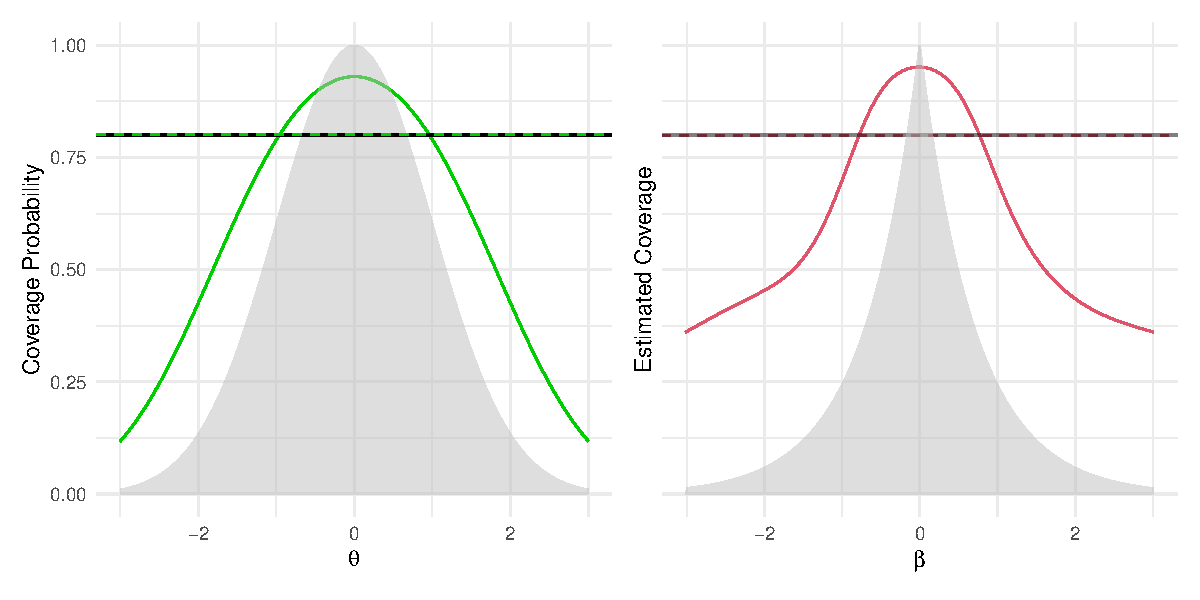
\includegraphics[width=0.8\linewidth]{figure1}
  \caption{\label{Fig:laplace} The left side of the figure provides coverage probabilities of Ridge CIs for a range of $\theta$ values as described in Section~\ref{Sec:difficulties}. The right side of the figure display results from the simulation described in Section~\ref{Sec:coverage}. For the right side of the figure, the fitted curve is from a Binomial GAM fit with coverage being modeled as a smooth function of $\beta$. The dashed line represent the average for the RL-P across all 1000 independently generated datasets and the solid black line indicates the nominal coverage rate. The shaded distribution in the background depicts the Laplace distribution the $\beta$s were drawn from. The analogous lines in the left side of the figure are exact calculations with the shaded normal in the background representing the prior.}
  \end{center}
\end{figure}

\begin{figure}[htb!]
  \begin{center}
  \includegraphics[width=0.7\linewidth]{figure2}
  \caption{\label{Fig:ridge_converge} Average coverages across p parameters (dashed lines) and estimated coverages as functions of $\beta$ (solid curves) for intervals constructed using a pairs bootstrap (Ridge Bootstrap) and a Bayesian posterior (Ridge). Full details of the simulation set up can be found in Section~\ref{Sec:boot-bias}.}
  \end{center}
\end{figure}

\begin{figure}[htb!]
  \begin{center}
  \includegraphics[width=0.8\linewidth]{figure3}
  \caption{\label{Fig:correlation_structure} This figure presents results for the simulation described in Section~\ref{Sec:correlation}. The violin plots are for the coverage rates across 1000 simulated datasets for the RL-P method and across three different levels of autoregressive correlation among the covariates, $\rho = 0 \text{ (no correlation)}, 0.5, 0.8$. For this simulation, p = 100, and the results for each level of correlation are presented across four different sample sizes, n = $\frac{1}{2}$p, p, 4p, 10p. The horizontal black line provides reference for the 80\% nominal coverage rate.}
  \end{center}
\end{figure}

\begin{table}[htb!]
  \centering
  \input{code/out/table1}
  \caption{\label{Tab:dist_beta} Results are from the simulation described in Section~\ref{Sec:distribution}. The nominal coverage rate is 80\%.}
\end{table}


\begin{figure}[htb!]
  \begin{center}
  \includegraphics[width=0.6\linewidth]{figure4.png}
  \caption{\label{Fig:beta_lambda_heatmap_laplace} The heatmap displays relative coverage for RL-P across a range of $\lambda$s per the simulation described in Section~\ref{Sec:lambda}. A Binomial GAM was used to estimate coverage as a smooth function of the $|\beta|$ and $\lam$. The x-axis for $\lambda$ is presented relative to $\lam_{\max}$ and the solid black lines indicate the center 95\% of $\lam_{\CV}$s over the 1000 simulations. The dashed black line indicates the median $\lambda_{\CV}$ and the blue line represents the value of $\lambda$ which provided coverage closest to that of nominal.}
  \end{center}
\end{figure}

\begin{figure}[htb!]
  \begin{center}
  \includegraphics[width=0.8\linewidth]{figure5}
  \caption{\label{Fig:highcorr} Provides results for simulation described in Section~\ref{Sec:Ridge}. The right plots show a single example of a intervals produced by Ridge (top) and RL-P (bottom) from one (randomly selected) of the 1000 datasets for the first 20 variables. The left plot summarizes the resulting CIs for the variables $A$, $B$, and $N1$ across the 1000 simulations. All 1000 CIs are plotted, sorted by their midpoint, with those colored red that did not contain contain the true coefficient value (indicated by the horizontal dashed gold line).}
  \end{center}
\end{figure}

\begin{figure}[htb!]
  \begin{center}
    \includegraphics[width=0.55\linewidth]{figure6}
    \caption{\label{Fig:laplace_comparison} Results are from the simulation described in Section~\ref{Sec:Comparison} and identical in setup to that of Section~\ref{Sec:coverage}. The fitted curves are from Binomial GAMs fit with coverage being modeled as a smooth function of $\beta$. The dashed lines represent the average coverage for each method across all 1000 independently generated datasets and the solid black line indicates the nominal coverage rate. The shaded distribution in the background depicts the Laplace distribution the $\beta$s were drawn from.}
  \end{center}
\end{figure}

\begin{figure}[htb!]
  \begin{center}
    \includegraphics[width=0.7\linewidth]{figure7}
    \caption{\label{Fig:laplace_other} Results are from the simulation described in Section~\ref{Sec:Comparison}. Each plot provides corresponding results for each of de-sparsified lasso, RL-P, and Selective Inference for three different sample sizes. The top provides violin plots of average coverages, the middle is a bar plot of the the median CI widths, and the bottom is a bar plot of the average run times, across all 1000 simulated datasets. The y limits have been truncated for the median width from 150 to 20.}
  \end{center}
\end{figure}

\begin{figure}[htb!]
  \begin{center}
    \includegraphics[width=0.9\linewidth]{figure8}
    \caption{\label{Fig:comparison_data_whoari} Confidence intervals produced by three different methods for all 66 variables in the WHO-ARI dataset described in Section~\ref{Sec:WHO-ARI}.}
  \end{center}
\end{figure}


\begin{table}[htb!]
  \centering
  \input{code/out/tableS1}
  \caption{Additional information on the results for Selective Inference in the simulation described in Section~\ref{Sec:Comparison}.}
\end{table}

